\documentclass[
../../EiKI_Summary.tex,
]
{subfiles}
    
\externaldocument[ext:]{../../EiKI_Summary.tex}
% Set Graphics Path, so pictures load correctly
\graphicspath{{../../}}

\begin{document}
\section{Machine Ethics}
\subsection{Concerns}
\subsubsection{Biases}
AI systems are inherently biased, because the data they're trained on is too. One small detail can yield entirely different results.

\begin{figure}
    [H]
    \centering
    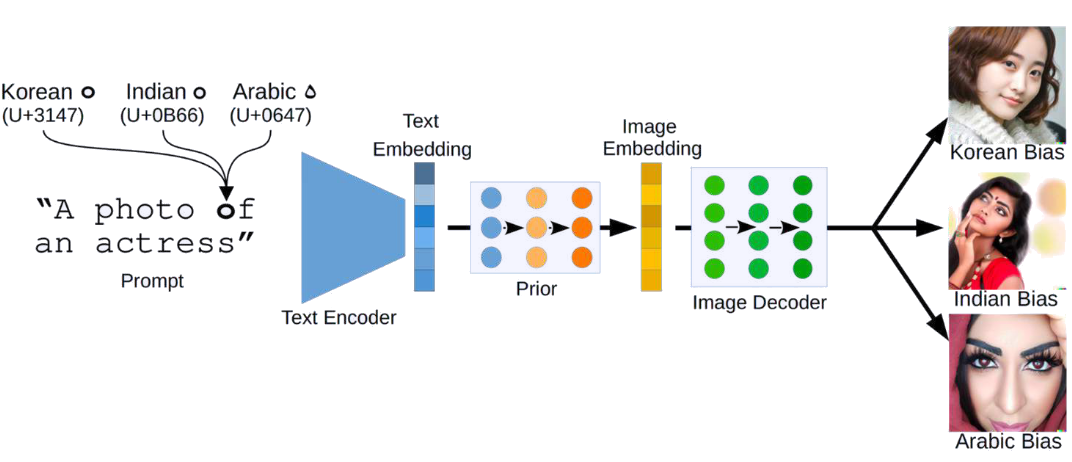
\includegraphics[width=0.6\textwidth]{Pics/10/BiasExample.png}
    \caption{Bias in Text-to-Image}
\end{figure}

\subsubsection{Data Privacy}
Due to the large amounts of data an AI is usually trained on, it is almost inevitable that this data, and by extension the AI model, contains information that it shouldn't have. This may include leaked personal information and the likes, but also things like simply being able to recognize people it isn't trained for. 

If we wanted to train a model to be able to recognize one specific person we also have to feed it data that doesn't contain that person. This causes the program to also being able to detect other persons.

\subsubsection{Causal Reasoning without Causality}
LLMs work on a mostly probabilistic basis. This means that they calculate the string of words that is most likely to correspond to the input. By doing this they mimic the causal reasoning of the data they're trained on, but do not actually employ causal connections. 

This leads to a false sense of security when asking LLMs about factual information.

\subsection{Mitigation of Concerns}
\subsubsection{Make AI systems aware of unwanted behaviour}
We can try to mitigate the problem of biases by trying to train AI on data that is as unbiased as possible. This, of course, is incredibly hard to do, as AI models need a large amount of data, which is hard to moderate. 

Another option is to implement filters. For example, we can implement a filter that makes it impossible to produce pornographic pictures of specific persons, or try to ''rework'' the result into something better.

Another thing we can do is \defc{train models to be able to detect biases and concerns} (revision engine). Once again, this is hard to do, as first you need to find out what biases and concerns exist, and then train models to detect them and answer responsibly. This results in a long process, that is often still ongoing when an AI is deployed and continues until it is discontinued.

Often \defc{reasoning} models are used for this. If we are able to make an AI be able to explain the reasoning behind its answer, it is more likely to detect when it is doing something it shouldn't.
\end{document}